\subsection{Recommendation}
\label{sec:Suggestion:Recommendation}

Wheras an \textsf{Operator} concerns \textsf{MM}, a \textsf{Recommendation} 
describes an action a methodologist may perform on \textsf{VT} in order to
co-evolve \viewtypes. 
In our approach, we issue a \textsf{Recommendation} for each \viewtype element 
impacted by an \textsf{Operator}. We identified four kinds of \textsf{Action}s: 
\begin{itemize}
	\item a \textsf{DEL}ete action that a \viewtype element is no longer associated
	to an \textsf{MM} element, and thus may be deleted;
	\item an \textsf{ADD} action suggests to create a new element in the \viewtype
	to reflect a newly created \textsf{MM} element;
	\item an \textsf{UP}date action changes the (String) value of a \viewtype element;
	\item a \textsf{MOVE} action suggests to move a \viewtype element from a \textsf{src}
	(source) to \textsf{tgt} (target) container.
\end{itemize}
Note that each \textsf{Recommendation} action stores a \textsf{name} (which corresponds
to the new value for \textsf{UP}date, whereas \textsf{previous} indicates the original
one) as well as its \textsf{container}, but also indicates the \textsf{type} of the
\viewtype meta-element on which the \textsf{Recommendation} is performed.

\autoref{tab:suggestions} provides the details of each \textsf{Recommendation} 
following the list of \textsf{Operator}s we identified in Sec. 
\ref{sec:Suggestion:Change} and commented in the next section.

\begin{figure}[t]
    \centering
    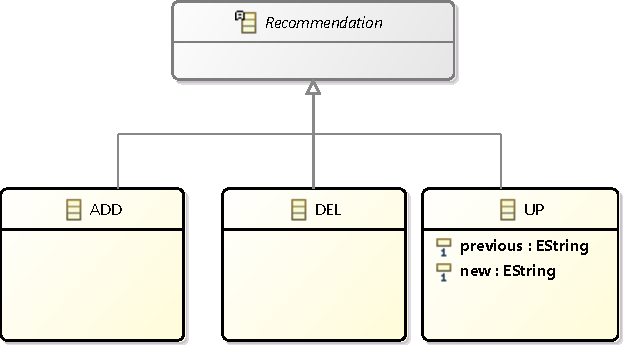
\includegraphics[width=\columnwidth]{Recommendation.pdf}
    \caption{\textsf{Recommendation}s suggested after a \textsf{Change}
    e.g. in Step 1, \textsf{ADD} Attribute \textsf{name} in \textsf{Transition}}
    \label{fig:Recommendation}
\end{figure}